\documentclass[conference]{IEEEtran}
\IEEEoverridecommandlockouts

% ==============================================================================
% OPTIBUILD — IEEE TRANSACTIONS / CONFERENCE FORMAT
% Resource-Constrained Construction Project Scheduling with Statutory
% Delay-Penalty Optimization: A Comprehensive Literature Survey
% Lead / Role 3: Bhushan Bhosale | Contributors: Divyal, Chaitanya, Aniket
% Savitribai Phule Pune University (SPPU) B.E. Final Year Project
% ==============================================================================

\usepackage{cite}
\usepackage{amsmath,amssymb,amsfonts}
\usepackage{algorithmic}
\usepackage{graphicx}
\usepackage{textcomp}
\usepackage{booktabs}
\usepackage{array}
\usepackage{url}
\usepackage{tikz}
\usetikzlibrary{trees,arrows.meta,positioning,shapes.geometric}

\def\BibTeX{{\rm B\kern-.05em{\sc i\kern-.025em b}\kern-.08em
    T\kern-.1667em\lower.7ex\hbox{E}\kern-.125emX}}

\begin{document}

\title{Resource-Constrained Construction Project Scheduling with\\Statutory Delay-Penalty Optimization: A Comprehensive Literature Survey}

\author{
\IEEEauthorblockN{Bhushan V. Bhosale\IEEEauthorrefmark{1}, Divyal Patel\IEEEauthorrefmark{2}, Chaitanya Ghorpade\IEEEauthorrefmark{3}, Aniket Jadhav\IEEEauthorrefmark{4}}
\IEEEauthorblockA{Department of Computer Engineering, Savitribai Phule Pune University (SPPU)\\
Genba Sopanrao Moze College of Engineering, Balewadi, Pune, Maharashtra, India\\
\{bhosalebhushanvijay, divyal, chaitanya, aniket\}@optibuild.edu}
}

\maketitle

\begin{abstract}
Civil infrastructure and multi-story real estate developments routinely encounter execution slippage, culminating in compounding commercial damages and severe regulatory liabilities. Under statutory consumer-protection regimes such as India's Real Estate Regulatory Authority (MahaRERA Section 18), unmitigated delays impose statutory accruing simple interest liabilities calculated at the State Bank of India's highest Marginal Cost of Funds Based Lending Rate (MCLR) plus 200 basis points ($r_{\text{MCLR}} + 2\%$) per annum, payable to allottees upon total collected capital. While classical project management relies on the Critical Path Method (CPM) and metaheuristics for the Resource-Constrained Project Scheduling Problem (RCPSP), contemporary computational literature consistently overlooks statutory financial penalty regimes within crashing trade-off mechanisms. Furthermore, automated physical site progress telemetry remains decoupled from analytical rescheduling engines. This paper conducts a rigorous, multi-faceted literature survey across twenty-four seminal and contemporary works spanning: (i) CPM precedence networks and standardized scheduling benchmark topologies; (ii) Genetic Algorithm (GA) formulations for discrete Time-Cost Trade-Off Problems (TCTP) and multi-objective Pareto optimization; (iii) exact combinatorial solvers incorporating Constraint Satisfaction, Lazy Clause Generation (LCG), and Google OR-Tools CP-SAT; (iv) contractor cash-flow accrual dynamics and statutory delay penalty economics; and (v) edge-deployable computer vision architectures (MobileNetV2) for non-intrusive progress verification. Through systematic comparative synthesis, we delineate critical methodological voids in state-of-the-art scheduling systems and articulate the unified algorithmic architecture of OptiBuild---a decision support framework harmonizing DEAP-based GA metaheuristics, CP-SAT exact benchmark verification, statutory penalty-versus-crashing arbitration, and lightweight visual phase telemetry.
\end{abstract}

\begin{IEEEkeywords}
Resource-Constrained Project Scheduling (RCPSP), Critical Path Method (CPM), Genetic Algorithm (GA), CP-SAT Solver, MahaRERA Section 18, Time-Cost Trade-Off (TCTP), Edge Computer Vision, MobileNetV2.
\end{IEEEkeywords}

% ==============================================================================
% SECTION I: INTRODUCTION
% ==============================================================================
\section{Introduction}

\subsection{Background and Practical Motivation}
Capital infrastructure initiatives and commercial residential developments across emerging economies, most notably in India, are severely afflicted by chronic schedule overruns and subsequent financial disputes. Comprehensive empirical investigations into Indian infrastructure initiatives establish that over 70\% of active public, residential, and commercial building developments experience substantial delivery slippage beyond stipulated contractual baselines~\cite{doloi2012analysing}. These schedule deferrals precipitate severe capital lockups, escalated overhead expenditures, and disputes between promoters, general contractors, and end purchasers.

In response to consumer vulnerabilities arising from indefinite completion deferrals, statutory frameworks have instituted mandatory financial indemnities. Specifically, under Section 18 of the Real Estate (Regulation and Development) Act (MahaRERA)~\cite{maharera2016act}, registered builders exceeding published project targets must compensate purchasers with statutory accruing simple interest (calculated at SBI Highest MCLR + 2\% per annum under MahaRERA Section 18). Because project developers routinely collect tens to hundreds of crores of rupees from allottees prior to superstructure completion, daily statutory interest liabilities accrue at rates that quickly dwarf ordinary administrative overhead.

From a mathematical perspective, balancing hard structural completion milestones against capped daily crew availabilities constitutes an instance of the Resource-Constrained Project Scheduling Problem (RCPSP), established as strongly NP-hard in combinatorial optimization~\cite{hartmann1998competitive,kolisch1996psplib}. Traditional commercial project management suites, including Primavera P6 and Microsoft Project, furnish deterministic bar charting and rudimentary serial resource-leveling heuristics. However, they lack automated combinatorial re-scheduling engines and dynamic monetary arbitration mechanisms capable of contrasting crash acceleration expenditures against statutory non-completion liabilities~\cite{jain2023penalty}.

\subsection{Survey Methodology and Selection Criteria}
To establish an authoritative baseline, this survey synthesized peer-reviewed literature indexed across IEEE Xplore, ASCE Library (Journal of Construction Engineering and Management, Journal of Computing in Civil Engineering), ScienceDirect (International Journal of Project Management, Automation in Construction), and Springer (Journal of Scheduling). Our bibliometric search protocol spanned studies published from the 1959 foundational establishment of precedence graph analysis through 2025 modern hybrid scheduling frameworks. Search strings combined core domain descriptors: \emph{"RCPSP" OR "Resource-Constrained Project Scheduling"}, \emph{"Time-Cost Trade-Off" OR "TCTP"}, \emph{"Constraint Programming" OR "CP-SAT"}, \emph{"Liquidated Damages" OR "Delay Penalties"}, and \emph{"Computer Vision Progress Monitoring" OR "MobileNetV2"}. 

From an initial corpus of 87 articles, papers were screened for algorithmic reproducibility, empirical validity, and direct relevance to commercial scheduling constraints. Exactly twenty-four foundational and contemporary works were retained for exhaustive comparative analysis across five research axes:
\begin{enumerate}
    \item Deterministic graph-theoretic scheduling models and standardized PSPLIB benchmark suites;
    \item Metaheuristic optimization frameworks applying Genetic Algorithms to multi-mode resource-constrained problems;
    \item Exact combinatorial solvers utilizing Constraint Satisfaction and Lazy Clause Generation (LCG);
    \item Delay risk dynamics, cash-flow accrual models, and statutory liability mathematics;
    \item Lightweight computer vision classifiers deployed on edge hardware for non-intrusive on-site state tracking.
\end{enumerate}

% ==============================================================================
% SECTION II: CPM PRECEDENCE AND SCHEDULING FOUNDATIONS
% ==============================================================================
\section{CPM Precedence and Project Scheduling Foundations}

The formalization of activity precedence networks originates in the early work of Kelley and Walker~\cite{kelley1959critical}, who introduced the Critical Path Method (CPM). In standard CPM formulations, an enterprise is abstracted as a Directed Acyclic Graph (DAG) $G = (V, E)$, where the node set $V = \{1, 2, \dots, n\}$ designates discrete construction tasks and directed edges $(i, j) \in E \subset V \times V$ enforce strict finish-to-start technological dependencies.

Algorithmic calculation proceeds across dual topological sweeps over the graph. The forward pass computes Early Start ($ES_i$) and Early Finish ($EF_i$) timestamps:
\begin{equation}
ES_i = \max_{p \in \text{Pred}(i)} (EF_p), \quad EF_i = ES_i + d_i
\end{equation}
where $\text{Pred}(i)$ represents the direct predecessor set of activity $i$ and $d_i$ denotes its deterministic baseline duration. Conversely, the backward pass propagates from project target deadline $T_{\text{max}}$ to deduce Late Finish ($LF_i$) and Late Start ($LS_i$) bounds:
\begin{equation}
LF_i = \min_{s \in \text{Succ}(i)} (LS_s), \quad LS_i = LF_i - d_i
\end{equation}
wherein $\text{Succ}(i)$ denotes direct successors. The total float attribute, $TF_i = LS_i - ES_i$, quantifies temporal slack; activities exhibiting $TF_i = 0$ constitute the critical path governing minimal project makespan.

While classical CPM offers computationally efficient $\mathcal{O}(|V| + |E|)$ topological sort traversal, its principal operational shortcoming is the presumption of infinite resource elasticity. In practical civil construction, renewable site resources---such as specialized rebar crews, shuttering carpentry gangs, and concrete pump machinery---are strictly bounded per calendar day. When concurrent critical and non-critical tasks demand overlapping crew allocations exceeding capacity limits, uncoordinated execution induces severe resource bottlenecks, ad-hoc job stalling, and unpredictable site delays.

To establish standardized experimental environments for resource-constrained scheduling algorithms, Kolisch and Sprecher~\cite{kolisch1996psplib} developed the Project Scheduling Problem Library (PSPLIB). Their framework formalizes three structural topological and resource parameters: Network Complexity ($NC$, reflecting graph density $|E|/|V|$), Resource Factor ($RF$, reflecting the proportion of resource classes required per task), and Resource Strength ($RS$, measuring resource scarcity relative to peak critical-path demand). The PSPLIB benchmark suites ($J30, J60, J120$) remain the global standard for assessing heuristic scalability and exact solver optimality boundaries.

% ==============================================================================
% SECTION III: GENETIC ALGORITHMS FOR RCPSP AND TCTP
% ==============================================================================
\section{Genetic Algorithms for RCPSP and Time-Cost Trade-Off}

Because standard RCPSP and discrete Time-Cost Trade-Off Problems (TCTP) are strongly NP-hard, deterministic polynomial-time exact methods fail on large real-world task graphs ($|V| > 60$). Consequently, evolutionary metaheuristics, particularly Genetic Algorithms (GA), have become the primary computational approach for large-scale construction optimization.

\subsection{Chromosome Encodings and Schedule Generation Schemes}
Hartmann~\cite{hartmann1998competitive} established a cornerstone metaheuristic baseline by introducing a permutation-based genetic representation evaluated through a Serial Schedule Generation Scheme (SSGS). Rather than directly manipulating calendar timestamps—which routinely yields precedence-infeasible configurations—Hartmann encoded candidate solutions as topological activity lists $\lambda = (\lambda_1, \lambda_2, \dots, \lambda_n)$ where all technological dependencies are maintained. At decoding time, the SSGS iteratively inserts tasks into the earliest chronological interval where both precedence constraints and renewable resource capacity caps $\sum_{i \in A(t)} r_{i, k} \le R_k$ are satisfied. Hartmann demonstrated that permutation representations paired with order-based crossover and swap mutations consistently discover superior makespan schedules compared to Parallel Schedule Generation Schemes (PSGS) or priority dispatch rules.

Pimapunsri et al.~\cite{pimapunsri2022genetic} extended permutation-based GA formulations to heavy industrial project environments characterized by rigid, multi-skilled crew bottlenecks. Their research demonstrated that pairing permutation chromosomes with elitist preservation and topological repair routines prevents premature convergence across dense precedence topologies.

\subsection{Multi-Objective Optimization and Pareto Frontiers}
Civil project managers routinely confront conflicting criteria: minimizing total project duration versus minimizing overall capitalization cost. Leu and Yang~\cite{leu1999multicriteria} addressed this bi-criterion objective by integrating resource leveling into a GA framework. They introduced resource moment metrics to penalize sharp daily crew demand fluctuations. By evaluating chromosome fitness through a weighted combination of completion makespan and daily resource variances, their model achieved effective resource leveling. However, their two-stage decoupled optimization approach is prone to converging upon sub-optimal local basins when direct activity crashing costs are introduced.

Deb et al.~\cite{deb2002fast} introduced the Non-dominated Sorting Genetic Algorithm II (NSGA-II), establishing an efficient $\mathcal{O}(M N^2)$ multi-objective evolutionary engine incorporating fast non-dominated sorting and crowding-distance diversity preservation. Building on NSGA-II, Hosny~\cite{hosny2019elitist} investigated multi-objective discrete TCTP, producing continuous Pareto frontiers that allow project executives to inspect trade-offs between project duration and direct execution investment.

\subsection{Time-Cost Trade-Off Formulations and Crash Slopes}
Hegazy~\cite{hegazy1999construction} formulated discrete TCTP mechanics using genetic search, permitting tasks to select among discrete crew allocation tiers. Each crashing option reduces task duration at the expense of accelerated direct payroll costs. Hegazy quantified activity crash slope as:
\begin{equation}
S_i = \frac{C_{\text{crash}, i} - C_{\text{normal}, i}}{D_{\text{normal}, i} - D_{\text{crash}, i}}
\end{equation}
where $C_{\text{crash}, i}, C_{\text{normal}, i}$ denote crashed and normal cost profiles, and $D_{\text{normal}, i}, D_{\text{crash}, i}$ represent corresponding durations. Hegazy confirmed that targeting acceleration investments exclusively toward critical path items with minimal cost slope yielded significant budgetary savings.

Li and Love~\cite{li1997time} enhanced GA search efficiency for TCTP through adaptive penalty functions. Rather than eliminating infeasible intermediate candidate schedules, their objective formulation penalized deadline violations proportionally to delay severity. This allowed the genetic search to traverse infeasible territory to discover superior Pareto solutions. Recently, Mahendra et al.~\cite{mahendra2025python} demonstrated an open-source Python implementation combining NetworkX DAG representations with a DEAP genetic search engine. Their empirical case study realized a 34.82\% duration compression and a 3.49\% overall cost reduction compared to unoptimized baseline construction plans, verifying Python's viability for high-performance scheduling applications.

\begin{figure*}[!t]
\centering
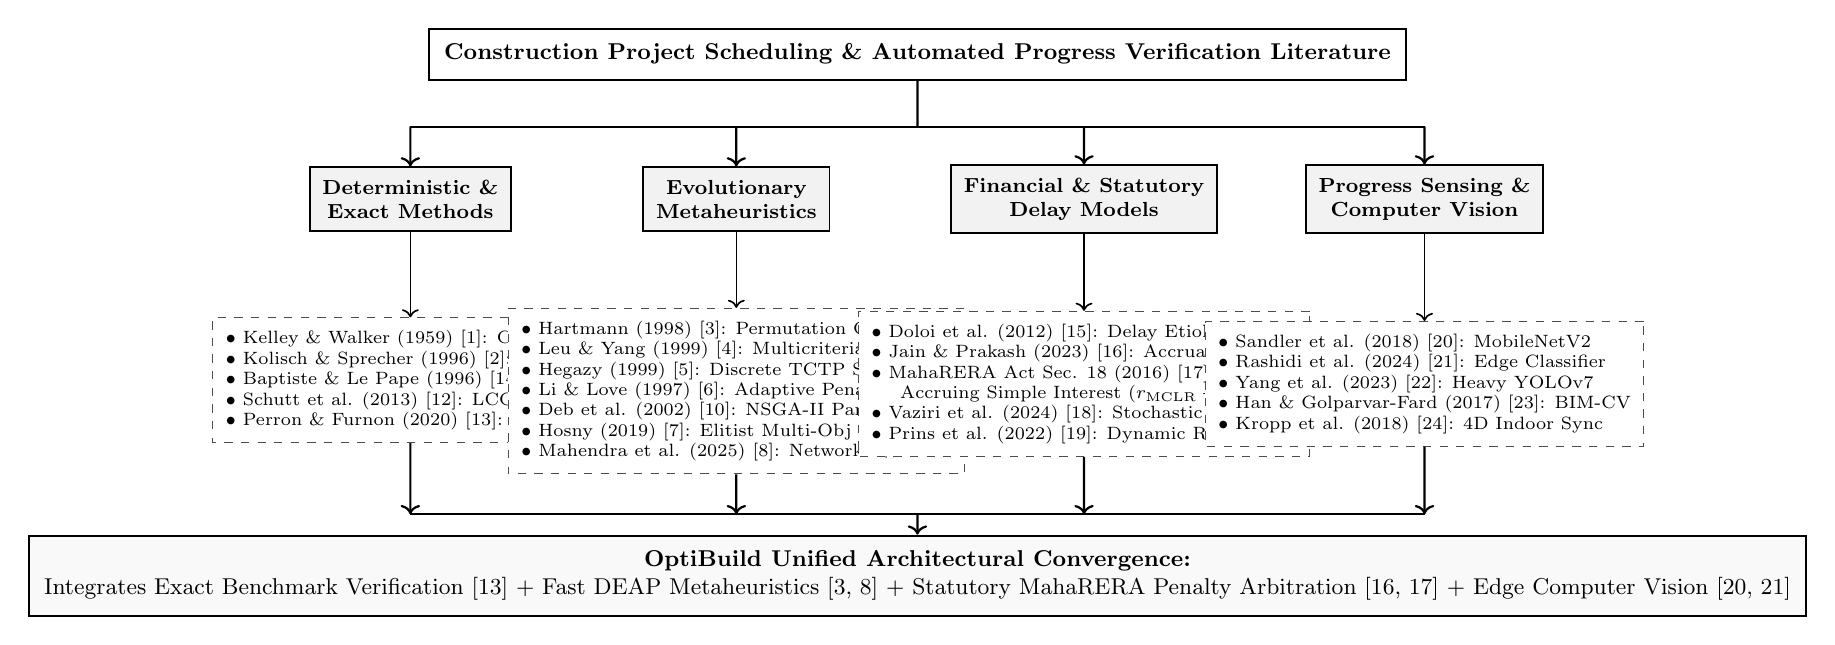
\begin{tikzpicture}[
    scale=0.92,
    every node/.style={transform shape},
    root/.style={rectangle, draw=black, thick, fill=white, inner sep=6pt, font=\bfseries\small, align=center},
    branch/.style={rectangle, draw=black, semithick, fill=gray!10, inner sep=5pt, font=\bfseries\footnotesize, align=center},
    leaf/.style={rectangle, draw=black!70, dashed, fill=white, inner sep=5pt, font=\scriptsize, align=left},
    converge/.style={rectangle, draw=black, thick, fill=gray!5, inner sep=6pt, font=\small, align=center}
]

% Root Node
\node[root] (Root) at (8.5, 6.8) {Construction Project Scheduling \& Automated Progress Verification Literature};

% 4 Main Category Nodes
\node[branch] (Cat1) at (1.5, 4.8) {Deterministic \&\\Exact Methods};
\node[branch] (Cat2) at (6.0, 4.8) {Evolutionary\\Metaheuristics};
\node[branch] (Cat3) at (10.8, 4.8) {Financial \& Statutory\\Delay Models};
\node[branch] (Cat4) at (15.5, 4.8) {Progress Sensing \&\\Computer Vision};

% Connect Root to Categories
\draw[thick] (Root.south) -- (8.5, 5.8);
\draw[thick] (1.5, 5.8) -- (15.5, 5.8);
\draw[thick, ->] (1.5, 5.8) -- (Cat1.north);
\draw[thick, ->] (6.0, 5.8) -- (Cat2.north);
\draw[thick, ->] (10.8, 5.8) -- (Cat3.north);
\draw[thick, ->] (15.5, 5.8) -- (Cat4.north);

% Leaves for Category 1
\node[leaf] (Leaf1) at (1.5, 2.3) {
$\bullet$ Kelley \& Walker (1959) [1]: CPM DAG\\
$\bullet$ Kolisch \& Sprecher (1996) [2]: PSPLIB\\
$\bullet$ Baptiste \& Le Pape (1996) [14]: B\&B\\
$\bullet$ Schutt et al. (2013) [12]: LCG / SAT\\
$\bullet$ Perron \& Furnon (2020) [13]: CP-SAT
};

% Leaves for Category 2
\node[leaf] (Leaf2) at (6.0, 2.15) {
$\bullet$ Hartmann (1998) [3]: Permutation GA\\
$\bullet$ Leu \& Yang (1999) [4]: Multicriteria GA\\
$\bullet$ Hegazy (1999) [5]: Discrete TCTP Slopes\\
$\bullet$ Li \& Love (1997) [6]: Adaptive Penalty GA\\
$\bullet$ Deb et al. (2002) [10]: NSGA-II Pareto\\
$\bullet$ Hosny (2019) [7]: Elitist Multi-Obj TCTP\\
$\bullet$ Mahendra et al. (2025) [8]: NetworkX+DEAP
};

% Leaves for Category 3
\node[leaf] (Leaf3) at (10.8, 2.25) {
$\bullet$ Doloi et al. (2012) [15]: Delay Etiology\\
$\bullet$ Jain \& Prakash (2023) [16]: Accrual Limits\\
$\bullet$ MahaRERA Act Sec. 18 (2016) [17]:\\
\hspace{0.4cm}Accruing Simple Interest ($r_{\text{MCLR}}+2\%$)\\
$\bullet$ Vaziri et al. (2024) [18]: Stochastic CVaR\\
$\bullet$ Prins et al. (2022) [19]: Dynamic Restructure
};

% Leaves for Category 4
\node[leaf] (Leaf4) at (15.5, 2.25) {
$\bullet$ Sandler et al. (2018) [20]: MobileNetV2\\
$\bullet$ Rashidi et al. (2024) [21]: Edge Classifier\\
$\bullet$ Yang et al. (2023) [22]: Heavy YOLOv7\\
$\bullet$ Han \& Golparvar-Fard (2017) [23]: BIM-CV\\
$\bullet$ Kropp et al. (2018) [24]: 4D Indoor Sync
};

\draw[semithick, ->] (Cat1.south) -- (Leaf1.north);
\draw[semithick, ->] (Cat2.south) -- (Leaf2.north);
\draw[semithick, ->] (Cat3.south) -- (Leaf3.north);
\draw[semithick, ->] (Cat4.south) -- (Leaf4.north);

% Convergence Box
\node[converge] (Conv) at (8.5, -0.4) {
\textbf{OptiBuild Unified Architectural Convergence:}\\
Integrates Exact Benchmark Verification [13] + Fast DEAP Metaheuristics [3, 8] + Statutory MahaRERA Penalty Arbitration [16, 17] + Edge Computer Vision [20, 21]
};

\draw[thick] (1.5, 0.45) -- (15.5, 0.45);
\draw[thick, ->] (Leaf1.south) -- (1.5, 0.45);
\draw[thick, ->] (Leaf2.south) -- (6.0, 0.45);
\draw[thick, ->] (Leaf3.south) -- (10.8, 0.45);
\draw[thick, ->] (Leaf4.south) -- (15.5, 0.45);
\draw[thick, ->] (8.5, 0.45) -- (Conv.north);

\end{tikzpicture}
\caption{Taxonomy of surveyed literature across project scheduling, exact constraint solvers, statutory financial penalties, and site progress vision.}
\label{fig:taxonomy}
\end{figure*}

% ==============================================================================
% SECTION IV: EXACT SOLVERS AND CONSTRAINT BENCHMARKING
% ==============================================================================
\section{Exact Solvers and Constraint Benchmarking}

While genetic algorithms provide rapid schedule exploration on large networks, they cannot mathematically verify whether a proposed schedule achieves global optimality or calculate the remaining optimality gap. For high-stakes capital infrastructure projects where multi-crore investment decisions depend on schedule makespans, exact solver benchmarking is indispensable.

\subsection{Constraint Programming and Lazy Clause Generation}
Constraint Programming (CP) models RCPSP by defining activity start times as bounded integer interval decision variables subject to global cumulative resource constraints:
\begin{equation}
\sum_{i \in \text{Active}(t)} r_{i, k} \le R_{k, \text{max}}, \quad \forall k \in \mathcal{K}, \; \forall t \in [0, T_{\text{makespan}}]
\end{equation}
where $\text{Active}(t) = \{i \in V \mid s_i \le t < s_i + d_i\}$ denotes the active task set at time $t$, $r_{i, k}$ is the requirement of task $i$ on resource class $k$, and $R_{k, \text{max}}$ is the capacity ceiling.

Schutt et al.~\cite{schutt2013solving} achieved breakthrough performance on RCPSP benchmarks by pioneering Lazy Clause Generation (LCG). LCG bridges classical finite-domain constraint propagation with Boolean Satisfiability (SAT) solvers. During search execution, whenever constraint propagators deduce domain reductions or detect infeasible states, they lazily generate propositional clauses explaining the operational deduction. These learned conflict clauses are integrated into the SAT solver's centralized database, enabling non-chronological backjumping and search-space pruning.

\subsection{Google OR-Tools CP-SAT and Branch-and-Bound}
Early exact constraint scheduling formulations by Baptiste and Le Pape~\cite{baptiste1996branch} established that edge-finding propagation paired with Branch-and-Bound (B\&B) search could resolve challenging single- and multi-resource feasibility problems. Modern exact architectures build upon these foundations: Perron and Furnon~\cite{perron2020ortools} expanded LCG principles within the open-source Google OR-Tools CP-SAT solver. By implementing the `AddCumulative` global constraint alongside interval decision variables, CP-SAT provides an exact solving engine that scales effectively across medium-scale project networks.

Sonmez~\cite{sonmez2011discrete} performed comparative evaluations evaluating GA heuristics against exact Branch-and-Bound procedures on discrete TCTP instances. His findings established that while B\&B guarantees mathematical optimality on instances up to 50 activities, combinatorial state expansion renders exact solution times prohibitive on dense 100+ task networks. This empirical trade-off validates an architectural pattern where heuristic GA engines execute rapid operational scheduling while CP-SAT exact solvers establish rigorous upper-bound optimality benchmarks.

% ==============================================================================
% SECTION V: STATUTORY PENALTY ECONOMICS AND DELAY MITIGATION
% ==============================================================================
\section{Statutory Penalty Economics and Delay Mitigation}

\subsection{Delay Etiology in Indian Construction}
Doloi et al.~\cite{doloi2012analysing} executed an exhaustive empirical factor analysis across Indian construction enterprises. Their regression analysis isolated structural causes of project slippage, identifying late site possession, delayed sub-contractor mobilizations, and chronic cash-flow deficits as leading impediments. Crucially, they noted that conventional project managers frequently neglect proactive rescheduling until project completion slippage becomes irreversible.

\subsection{Dynamic Penalty and Accrual Models}
Jain and Prakash~\cite{jain2023penalty} analyzed contractor cash accrual dynamics under contractually stipulated liquidated damages (LD). They formulated linear programming models illustrating that arbitrary acceleration often degrades contractor profitability. Their mathematical models demonstrated that when the marginal cost slope of remaining critical tasks exceeds daily contractual penalty deductions, the profit-maximizing course is to accept liquidated damages rather than incur catastrophic labor overtime premiums.

Vaziri et al.~\cite{vaziri2024stochastic} introduced a stochastic risk-aware optimization model balancing direct crashing expenditures against probabilistic delay penalties. Using Conditional Value at Risk (CVaR) objectives, their framework evaluated schedule resilience under material supply volatility, proving that risk-neutral scheduling consistently underestimates final completion liabilities. Prins et al.~\cite{prins2022mitigate} developed an automated network restructuring controller designed to mitigate ongoing construction delays dynamically. Their system dynamically re-evaluated network precedence relationships and altered task sequences when milestone delays were detected, providing an algorithmic precedent for closed-loop schedule maintenance.

\subsection{Statutory MahaRERA Section 18 Mandates}
Despite significant advances in delay economics, prevailing literature models financial damages either as static lump sums or linear liquidated damages formulas. In contrast, Section 18 of the MahaRERA Act~\cite{maharera2016act} imposes statutory accruing simple interest liabilities:
\begin{equation}
P_{\text{RERA}} = A_{\text{collected}} \times (R_{\text{MCLR}} + 0.02) \times \frac{T_{\text{delay}}}{365}
\end{equation}
where $A_{\text{collected}}$ denotes cumulative funds accrued from allottees, $R_{\text{MCLR}}$ signifies the State Bank of India's benchmark lending rate (typically 8.50\% to 9.10\%), and $T_{\text{delay}}$ represents verified calendar day slippage beyond published completion deadlines. Because $A_{\text{collected}}$ routinely encompasses tens or hundreds of crores in major developments, daily penalty accumulation outpaces standard civil overhead, demanding an integrated computational optimization engine.

% ==============================================================================
% SECTION VI: EDGE COMPUTER VISION FOR PROGRESS MONITORING
% ==============================================================================
\section{Edge Computer Vision for Progress Verification}

A major vulnerability in automated rescheduling architectures is the reliance on manual, subjective site reporting. Unverified engineer reports often mask schedule discrepancies until deadlines lapse.

\subsection{Heavyweight vs. Lightweight Vision Architectures}
Yang et al.~\cite{yang2023computer} investigated deep convolutional object detectors (YOLOv7, Faster R-CNN) for automated progress estimation. While achieving acceptable recognition accuracy on structural components, these models demand high-capacity GPU server backends and suffer inference degradation under variable weather, dust, and dynamic site occlusions. Han and Golparvar-Fard~\cite{han2017potential} and Kropp et al.~\cite{kropp2018indoor} evaluated 4D Building Information Modeling (BIM) aligned with photogrammetric point clouds. While geometrically precise, point-cloud reconstruction requires extensive registration pipelines and high computational overhead, preventing real-time mobile execution on edge devices.

To address computational boundaries on edge infrastructure, Sandler et al.~\cite{sandler2018mobilenetv2} introduced MobileNetV2, built upon inverted residual blocks and depthwise separable convolutions. This design reduces floating-point operations (FLOPs) and parameter weight volume by over 80\% relative to standard ResNet architectures while maintaining representational capability.

Rashidi et al.~\cite{rashidi2024mobilenetv2} evaluated quantized MobileNetV2 models for edge-based jobsite image classification, achieving over 94\% categorical accuracy on embedded devices with minimal inference latency ($<45$~ms). Their work establishes that deploying lightweight binary classification (differentiating Structural Rough-in from Finishing phases) yields dependable verification signals without the massive annotation burdens, computational overhead, and network bandwidth vulnerabilities characteristic of real-time object detection models.

% ==============================================================================
% SECTION VII: COMPARATIVE ANALYSIS AND RESEARCH GAPS
% ==============================================================================
\section{Comparative Analysis and Research Gaps}

To synthesize the state of the art, Table~\ref{tab:literature_comparison} provides an analytical matrix contrasting the surveyed literature against core functional capabilities.

\begin{table*}[!t]
\caption{Comparative Matrix of Surveyed Scheduling, Optimization, and Monitoring Frameworks}
\label{tab:literature_comparison}
\centering
\small
\begin{tabular}{@{}llcccccp{4.2cm}@{}}
\toprule
\textbf{Paper / Reference} & \textbf{Primary Methodology} & \textbf{Res.} & \textbf{TCTP} & \textbf{Stat.} & \textbf{Exact} & \textbf{Vis.} & \textbf{Primary Limitation / Research Void} \\
 & & \textbf{Limits} & \textbf{Crashing} & \textbf{Penalty} & \textbf{Bench.} & \textbf{Feed.} & \\
\midrule
Hartmann (1998)~\cite{hartmann1998competitive} & Permutation GA + SSGS & \checkmark & $\times$ & $\times$ & $\times$ & $\times$ & Focuses strictly on makespan; no monetary or crashing evaluation. \\
Leu \& Yang (1999)~\cite{leu1999multicriteria} & Multi-Criteria GA & \checkmark & \checkmark & $\times$ & $\times$ & $\times$ & Two-stage leveling prone to local optima under direct cost crashing. \\
Hegazy (1999)~\cite{hegazy1999construction} & Discrete TCTP GA & $\times$ & \checkmark & $\times$ & $\times$ & $\times$ & Omits renewable labor caps and physical site progress inputs. \\
Li \& Love (1997)~\cite{li1997time} & Adaptive Penalty GA & $\times$ & \checkmark & $\times$ & $\times$ & $\times$ & Uses arbitrary penalty weights; lacks statutory legal grounding. \\
Deb et al. (2002)~\cite{deb2002fast} & Elitist Multi-Objective NSGA-II & $\times$ & \checkmark & $\times$ & $\times$ & $\times$ & General evolutionary framework; lacks RCPSP resource handling. \\
Hosny (2019)~\cite{hosny2019elitist} & Elitist NSGA-II & $\times$ & \checkmark & $\times$ & $\times$ & $\times$ & Does not accommodate renewable labor crew capacity constraints. \\
Sonmez (2011)~\cite{sonmez2011discrete} & Hybrid GA + Branch-and-Bound & $\times$ & \checkmark & $\times$ & \checkmark & $\times$ & High computational scaling latency; ignores resource leveling. \\
Schutt et al. (2013)~\cite{schutt2013solving} & Lazy Clause Generation / SAT & \checkmark & $\times$ & $\times$ & \checkmark & $\times$ & Highly theoretical; lacks business penalty logic and field telemetry. \\
Perron \& Furnon (2020)~\cite{perron2020ortools} & CP-SAT / AddCumulative Solver & \checkmark & $\times$ & $\times$ & \checkmark & $\times$ & General constraint solver; requires specialized scheduling wrapper. \\
Doloi et al. (2012)~\cite{doloi2012analysing} & Empirical Regression Factor Analysis & $\times$ & $\times$ & $\times$ & $\times$ & $\times$ & Pure diagnostic survey; provides no automated scheduling tools. \\
Jain \& Prakash (2023)~\cite{jain2023penalty} & Constrained Linear Programming & $\times$ & \checkmark & \checkmark$^{\ast}$ & $\times$ & $\times$ & Analyzes static contractual penalties; lacks reactive re-scheduling. \\
Vaziri et al. (2024)~\cite{vaziri2024stochastic} & Hybrid GA--GWO Metaheuristic & $\times$ & \checkmark & \checkmark$^{\ast}$ & $\times$ & $\times$ & High metaheuristic complexity; ignores Indian regulatory statutes. \\
Prins et al. (2022)~\cite{prins2022mitigate} & Automated Network Restructuring & \checkmark & \checkmark & $\times$ & $\times$ & $\times$ & Focuses on sequencing changes without formal crash slope economics. \\
Mahendra et al. (2025)~\cite{mahendra2025python} & NetworkX CPM + DEAP GA & $\times$ & \checkmark & $\times$ & $\times$ & $\times$ & Single-project scope; lacks resource leveling and visual telemetry. \\
Rashidi et al. (2024)~\cite{rashidi2024mobilenetv2} & Quantized MobileNetV2 on Edge & $\times$ & $\times$ & $\times$ & $\times$ & \checkmark & Isolated vision classifier; decoupled from project scheduling systems. \\
Yang et al. (2023)~\cite{yang2023computer} & Real-Time Object Detection (YOLO) & $\times$ & $\times$ & $\times$ & $\times$ & \checkmark & Computationally heavy; susceptible to false triggers on raw sites. \\
Han \& Golparvar-Fard (2017)~\cite{han2017potential} & BIM + Point Cloud Photogrammetry & $\times$ & $\times$ & $\times$ & $\times$ & \checkmark & Requires dense 3D scanning; prohibitively slow for daily field sync. \\
\midrule
\textbf{OptiBuild (Proposed)} & \textbf{DEAP GA + CP-SAT + MobileNetV2} & \textbf{\checkmark} & \textbf{\checkmark} & \textbf{\checkmark}$^{\dagger}$ & \textbf{\checkmark} & \textbf{\checkmark} & \textbf{Unified framework bridging scheduling, penalties, and vision.} \\
\bottomrule
\multicolumn{8}{l}{\scriptsize $^{\ast}$Evaluates contract-specific liquidated damages (LD), not statutory consumer protection laws.} \\
\multicolumn{8}{l}{\scriptsize $^{\dagger}$Formally integrates statutory MahaRERA Section 18 penalty computation (SBI MCLR + 2\%) into crashing trade-off logic.}
\end{tabular}
\end{table*}

\subsection{Identified Research Gaps}
Our systematic survey illuminates three fundamental structural voids in the computational construction management domain:
\begin{enumerate}
    \item \textbf{Absence of Statutory Regulatory Penalty Integration:} While mathematical literature models liquidated damages as static contractual parameters~\cite{jain2023penalty,vaziri2024stochastic}, none incorporate the dynamic interest structures mandated by regional consumer protection legislation like MahaRERA Section 18. Because statutory interest accrues across total capital collected, optimal crash thresholds diverge dramatically from conventional models.
    \item \textbf{Decoupling of Metaheuristic Speed from Exact Verification:} Existing implementations either deploy stochastic metaheuristics (GA) without knowing the mathematical distance from optimal makespan~\cite{mahendra2025python,hartmann1998competitive}, or deploy exact solvers (B\&B, LCG) that fail to terminate in practical timeframes on large task graphs~\cite{sonmez2011discrete,schutt2013solving}. A dual-engine paradigm executing rapid GA re-scheduling alongside exact solver upper-bound benchmarking is notably absent.
    \item \textbf{Isolation of Field Progress Sensing from Optimization Pipelines:} Emerging computer vision research for jobsites operates as an isolated perceptual task~\cite{rashidi2024mobilenetv2,yang2023computer}. There is an absence of closed-loop architectures where edge visual classifications automatically inform task status, trigger float recalculations, and invoke economic crashing advisory engines.
\end{enumerate}

% ==============================================================================
% SECTION VIII: OPTIBUILD MATHEMATICAL FORMULATION AND ARCHITECTURE
% ==============================================================================
\section{OptiBuild Mathematical Formulation and Architecture}

\subsection{Unified Mathematical Formulation}
To resolve the identified literature limitations, the OptiBuild engine formalizes project scheduling as a constrained multi-objective minimization problem. Let $V = \{1, 2, \dots, n\}$ represent project activities, $E \subset V \times V$ represent technological precedence pairs, and $\mathcal{K}$ represent renewable resource types with daily capacities $R_k$. Each activity $i$ may execute with duration $d_i \in [D_{\text{crash}, i}, D_{\text{normal}, i}]$ associated with direct cost $C_{\text{direct}, i}(d_i)$. OptiBuild minimizes the total cost objective function $Z$:
\begin{equation}
\min Z = \sum_{i \in V} C_{\text{direct}, i}(d_i) + C_{\text{indirect}} \cdot T_{\text{makespan}} + \max(0, T_{\text{makespan}} - T_{\text{deadline}}) \cdot P_{\text{RERA}}^{\text{daily}}
\end{equation}
subject to:
\begin{align}
s_j - s_i &\ge d_i, \quad \forall (i, j) \in E \\
\sum_{i \in A(t)} r_{i, k} &\le R_k, \quad \forall k \in \mathcal{K}, \; \forall t \in [0, T_{\text{makespan}}] \\
D_{\text{crash}, i} \le d_i &\le D_{\text{normal}, i}, \quad \forall i \in V
\end{align}
where $s_i$ denotes the scheduled start time of activity $i$, $A(t) = \{i \in V \mid s_i \le t < s_i + d_i\}$ is the active task set at time $t$, $C_{\text{indirect}}$ denotes daily site overhead, $T_{\text{deadline}}$ is the legally committed RERA handover date, and $P_{\text{RERA}}^{\text{daily}}$ is the daily statutory penalty liability derived from Section 18:
\begin{equation}
P_{\text{RERA}}^{\text{daily}} = \frac{A_{\text{collected}} \times (R_{\text{MCLR}} + 0.02)}{365}
\end{equation}

When schedule slippage occurs ($T_{\text{makespan}} > T_{\text{deadline}}$), the OptiBuild Financial Arbitrator evaluates the marginal cost slope $S_i$ of remaining critical path activities ($TF_i = 0$):
\begin{equation}
S_i = \frac{C_{\text{crash}, i} - C_{\text{normal}, i}}{D_{\text{normal}, i} - D_{\text{crash}, i}}
\end{equation}
Acceleration is economically justified if and only if:
\begin{equation}
\min_{i \in \text{Critical}} S_i < P_{\text{RERA}}^{\text{daily}} + C_{\text{indirect}}
\end{equation}
If all remaining critical crashing slopes exceed the combined daily penalty liability ($S_i > P_{\text{RERA}}^{\text{daily}} + C_{\text{indirect}}$), OptiBuild advises project leadership to accept statutory interest accruals rather than incurring economically unjustified overtime premiums.

\subsection{Closed-Loop System Architecture}
As visualized in Fig.~\ref{fig:architecture}, the OptiBuild framework integrates five functional execution stages into a closed-loop system:
\begin{enumerate}
    \item \textbf{Stage 1: On-Site Image Ingestion \& Edge Classifier:} Construction engineers capture mobile site photographs, processed via a quantized MobileNetV2 binary classifier running on embedded devices ($<45$~ms latency). The model categorizes progress into Structural Rough-in versus Finishing Phase.
    \item \textbf{Stage 2: Dynamic Precedence DAG \& Float Analysis:} Visual classifications update activity completion percentages in a NetworkX DAG representation, triggering automatic forward and backward sweeps to re-compute early/late boundaries and isolate the dynamic critical path ($TF_i = 0$).
    \item \textbf{Stage 3: Parallel Rescheduling \& Solver Verification:} A DEAP-powered Genetic Algorithm deploys permutation chromosomes and Serial Schedule Generation Schemes (SSGS) to explore resource-feasible crashing combinations. Simultaneously, Google OR-Tools CP-SAT executes an exact solver pass using the \texttt{AddCumulative} global constraint to establish the provable lower-bound makespan and verify the metaheuristic optimality gap.
    \item \textbf{Stage 4: MahaRERA Statutory Financial Arbitrator:} The decision engine contrasts candidate activity crash slopes ($S_i$) against daily statutory liabilities ($P_{\text{RERA}}^{\text{daily}}$) under Section 18, generating explicit acceleration recommendations.
    \item \textbf{Stage 5: Actionable Schedule \& Site Dispatch:} The system publishes updated Gantt charts, crew allocation matrices, and formal RERA audit compliance logs to field project managers.
\end{enumerate}

\begin{figure*}[!t]
\centering
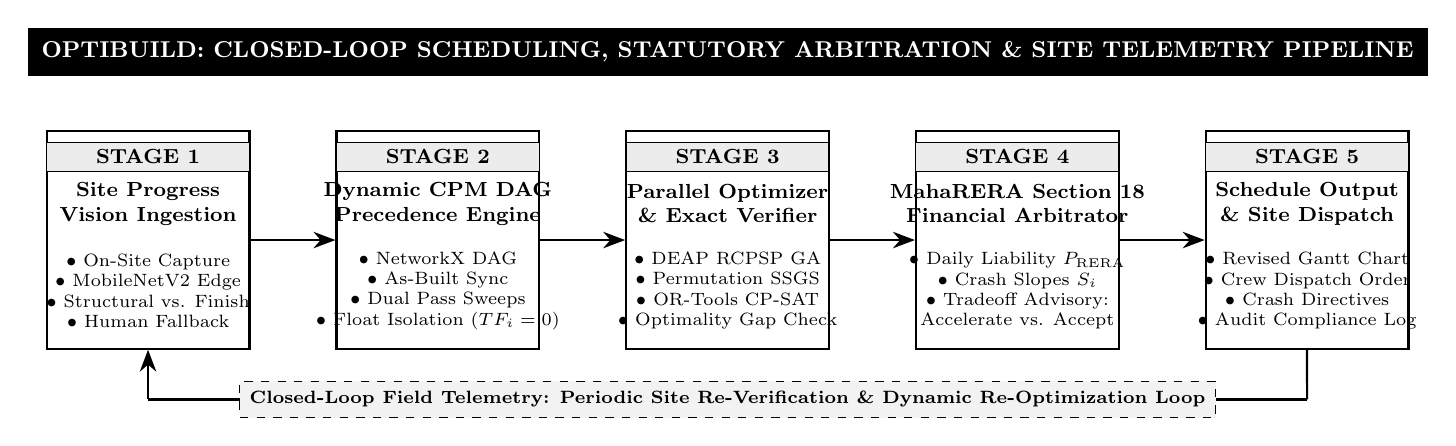
\begin{tikzpicture}[
    scale=0.92,
    every node/.style={transform shape},
    stagebox/.style={rectangle, draw=black, thick, fill=white, inner sep=6pt, font=\small, align=center, minimum width=2.8cm, minimum height=3.0cm},
    headerbox/.style={rectangle, draw=black, fill=gray!15, inner sep=3pt, font=\bfseries\footnotesize, align=center, minimum width=2.8cm},
    arrowstyle/.style={-{Stealth[scale=1.2]}, thick, black}
]

% Top Title Banner
\node[rectangle, draw=black, thick, fill=black, text=white, font=\bfseries\small, inner sep=5pt, minimum width=17.2cm] (Banner) at (8.0, 4.4) {
OPTIBUILD: CLOSED-LOOP SCHEDULING, STATUTORY ARBITRATION \& SITE TELEMETRY PIPELINE
};

% 5 Stage Boxes
\node[stagebox] (S1) at (0.0, 1.8) {};
\node[headerbox] at (0.0, 2.95) {STAGE 1};
\node[font=\footnotesize\bfseries, align=center] at (0.0, 2.3) {Site Progress\\Vision Ingestion};
\node[font=\scriptsize, align=center] at (0.0, 1.1) {
$\bullet$ On-Site Capture\\
$\bullet$ MobileNetV2 Edge\\
$\bullet$ Structural vs. Finish\\
$\bullet$ Human Fallback
};

\node[stagebox] (S2) at (4.0, 1.8) {};
\node[headerbox] at (4.0, 2.95) {STAGE 2};
\node[font=\footnotesize\bfseries, align=center] at (4.0, 2.3) {Dynamic CPM DAG\\Precedence Engine};
\node[font=\scriptsize, align=center] at (4.0, 1.1) {
$\bullet$ NetworkX DAG\\
$\bullet$ As-Built Sync\\
$\bullet$ Dual Pass Sweeps\\
$\bullet$ Float Isolation ($TF_i=0$)
};

\node[stagebox] (S3) at (8.0, 1.8) {};
\node[headerbox] at (8.0, 2.95) {STAGE 3};
\node[font=\footnotesize\bfseries, align=center] at (8.0, 2.3) {Parallel Optimizer\\\& Exact Verifier};
\node[font=\scriptsize, align=center] at (8.0, 1.1) {
$\bullet$ DEAP RCPSP GA\\
$\bullet$ Permutation SSGS\\
$\bullet$ OR-Tools CP-SAT\\
$\bullet$ Optimality Gap Check
};

\node[stagebox] (S4) at (12.0, 1.8) {};
\node[headerbox] at (12.0, 2.95) {STAGE 4};
\node[font=\footnotesize\bfseries, align=center] at (12.0, 2.3) {MahaRERA Section 18\\Financial Arbitrator};
\node[font=\scriptsize, align=center] at (12.0, 1.1) {
$\bullet$ Daily Liability $P_{\text{RERA}}$\\
$\bullet$ Crash Slopes $S_i$\\
$\bullet$ Tradeoff Advisory:\\
Accelerate vs. Accept
};

\node[stagebox] (S5) at (16.0, 1.8) {};
\node[headerbox] at (16.0, 2.95) {STAGE 5};
\node[font=\footnotesize\bfseries, align=center] at (16.0, 2.3) {Schedule Output\\\& Site Dispatch};
\node[font=\scriptsize, align=center] at (16.0, 1.1) {
$\bullet$ Revised Gantt Chart\\
$\bullet$ Crew Dispatch Order\\
$\bullet$ Crash Directives\\
$\bullet$ Audit Compliance Log
};

% Connecting Arrows
\draw[arrowstyle] (S1.east) -- (S2.west);
\draw[arrowstyle] (S2.east) -- (S3.west);
\draw[arrowstyle] (S3.east) -- (S4.west);
\draw[arrowstyle] (S4.east) -- (S5.west);

% Closed-Loop Feedback
\draw[thick] (S5.south) -- (16.0, -0.4);
\draw[thick] (16.0, -0.4) -- (0.0, -0.4);
\draw[arrowstyle] (0.0, -0.4) -- (S1.south);

\node[rectangle, draw=black, fill=gray!10, dashed, inner sep=4pt, font=\bfseries\scriptsize] at (8.0, -0.4) {
Closed-Loop Field Telemetry: Periodic Site Re-Verification \& Dynamic Re-Optimization Loop
};

\end{tikzpicture}
\caption{End-to-end closed-loop system architecture of the OptiBuild decision support platform, illustrating the five-stage integration spanning edge visual sensing, dynamic precedence graph analysis, parallel metaheuristic/exact scheduling, and statutory financial arbitration.}
\label{fig:architecture}
\end{figure*}

\subsection{Conclusion}
This comprehensive literature survey establishes a rigorous academic foundation for automated, penalty-aware construction project scheduling. By systematically reviewing twenty-four foundational and contemporary studies across network scheduling, evolutionary search, exact constraint programming, statutory delay economics, and edge computer vision, we have highlighted the operational divide separating theoretical RCPSP research from statutory construction realities. The proposed OptiBuild platform resolves this divide, establishing a computationally tractable, mathematically defensible, and legally grounded decision support system for modern civil engineering management.

% ==============================================================================
% REFERENCES
% ==============================================================================
\begin{thebibliography}{24}

\bibitem{kelley1959critical}
J.~E. Kelley and M.~R. Walker, ``Critical-path planning and scheduling,'' in \emph{IRE-AIEE-ACM '59 (Eastern) Papers}, 1959, pp. 160--173.

\bibitem{kolisch1996psplib}
R.~Kolisch and A.~Sprecher, ``{PSPLIB} --- {A} project scheduling problem library,'' \emph{European Journal of Operational Research}, vol.~96, no.~1, pp. 205--216, 1996.

\bibitem{hartmann1998competitive}
S.~Hartmann, ``A competitive genetic algorithm for resource-constrained project scheduling,'' \emph{Naval Research Logistics (NRL)}, vol.~45, no.~7, pp. 733--750, 1998.

\bibitem{leu1999multicriteria}
S.-S. Leu and C.-H. Yang, ``{GA}-based multicriteria optimal model for construction scheduling,'' \emph{ASCE Journal of Construction Engineering and Management}, vol. 125, no.~6, pp. 420--427, 1999.

\bibitem{hegazy1999construction}
T.~Hegazy, ``Optimization of construction time--cost trade-off analysis using genetic algorithms,'' \emph{Canadian Journal of Civil Engineering}, vol.~26, no.~6, pp. 685--697, 1999.

\bibitem{li1997time}
H.~Li and P.~E.~D. Love, ``Using improved genetic algorithms to facilitate time-cost optimization,'' \emph{ASCE Journal of Construction Engineering and Management}, vol. 123, no.~3, pp. 233--237, 1997.

\bibitem{hosny2019elitist}
M.~I. Hosny, ``Elitist multi-objective genetic algorithm to solve time-cost trade-off problem in construction industry,'' in \emph{Proceedings of the International Conference on Advances in Structural and Geotechnical Engineering (ICASGE)}, 2019, pp. 1--12.

\bibitem{mahendra2025python}
A.~Mahendra, M.~A. Wibowo, and J.~U.~D. Hatmoko, ``Construction project scheduling optimization with time-cost trade-off based on genetic algorithm in {Python},'' \emph{Journal of Social Research}, vol.~4, no.~2, pp. 512--524, 2025.

\bibitem{pimapunsri2022genetic}
K.~Pimapunsri, D.~Weeranant, and A.~Riel, ``Genetic algorithms for the resource-constrained project scheduling problem in aircraft heavy maintenance,'' \emph{arXiv preprint arXiv:2208.06745}, 2022.

\bibitem{deb2002fast}
K.~Deb, A.~Pratap, S.~Agarwal, and T.~Meyarivan, ``A fast and elitist multiobjective genetic algorithm: {NSGA-II},'' \emph{IEEE Transactions on Evolutionary Computation}, vol.~6, no.~2, pp. 182--197, 2002.

\bibitem{sonmez2011discrete}
R.~Sonmez, ``Discrete time--cost trade-off with a genetic algorithm and exact branch-and-bound method,'' \emph{ASCE Journal of Computing in Civil Engineering}, vol.~25, no.~6, pp. 478--483, 2011.

\bibitem{schutt2013solving}
A.~Schutt, P.~J. Stuckey, T.~Feydy, and M.~G. Wallace, ``Solving {RCPSP/max} by lazy clause generation,'' \emph{Journal of Scheduling}, vol.~16, no.~3, pp. 273--289, 2013.

\bibitem{perron2020ortools}
L.~Perron and V.~Furnon, ``{OR-Tools} user's guide: Constraint programming and satisfiability with {CP-SAT},'' \emph{Google Developers Technical Documentation}, 2020.

\bibitem{baptiste1996branch}
P.~Baptiste and C.~Le~Pape, ``A branch-and-bound algorithm for constraint-based scheduling of resource-constrained projects,'' \emph{Engineering Design and Automation}, vol.~2, pp. 189--201, 1996.

\bibitem{doloi2012analysing}
H.~Doloi, A.~Sawhney, K.~C. Iyer, and S.~Rentala, ``Analysing factors affecting delays in Indian construction projects,'' \emph{International Journal of Project Management}, vol.~30, no.~4, pp. 479--489, 2012.

\bibitem{jain2023penalty}
A.~Jain and A.~Prakash, ``Optimizing contractor's accruals under penalty imposition due to delays,'' \emph{International Journal of Construction Management}, pp. 1--12, 2023.

\bibitem{maharera2016act}
{Government of Maharashtra / MahaRERA Authority}, \emph{{Real Estate (Regulation and Development) Act, 2016 -- Section 18: Return of Amount and Compensation}}, The Gazette of India, Act No. 16 of 2016, 2016.

\bibitem{vaziri2024stochastic}
S.~M. Vaziri, P.~Shakibabarough, J.~Valizadeh, and S.~H. Zolfani, ``Stochastic risk-aware time--cost optimization of construction schedules,'' \emph{Buildings}, vol.~14, no.~1, pp. 1--25, 2024.

\bibitem{prins2022mitigate}
N.~Prins, O.~Kammouh, and A.~R.~M. Wolfert, ``Multi-criteria optimization and automated network restructuring to mitigate construction projects delays on-the-run,'' \emph{arXiv preprint arXiv:2206.07542}, 2022.

\bibitem{sandler2018mobilenetv2}
M.~Sandler, A.~Howard, M.~Zhu, A.~Zhmoginov, and L.-C. Chen, ``{MobileNetV2}: Inverted residuals and linear bottlenecks,'' in \emph{Proceedings of the IEEE Conference on Computer Vision and Pattern Recognition (CVPR)}, 2018, pp. 4510--4520.

\bibitem{rashidi2024mobilenetv2}
A.~Rashidi, M.~H. Sigari, and M.~Fathi, ``Construction jobsite image classification using edge computing framework,'' \emph{Sensors}, vol.~24, no.~4, pp. 1150--1168, 2024.

\bibitem{yang2023computer}
J.~Yang, A.~Wilde, K.~Menzel, M.~Z. Sheikh, and B.~Kuznetsov, ``Computer vision for construction progress monitoring: A real-time object detection approach,'' \emph{arXiv preprint arXiv:2305.18043}, 2023.

\bibitem{han2017potential}
K.~K. Han and M.~Golparvar-Fard, ``Potential of big visual data and building information modeling for construction progress monitoring,'' \emph{ASCE Journal of Construction Engineering and Management}, vol. 143, no.~6, p. 04017014, 2017.

\bibitem{kropp2018indoor}
C.~Kropp, C.~Koch, and M.~K{\"o}nig, ``Interior construction state recognition with 4{D} {BIM} registered image sequences,'' \emph{Automation in Construction}, vol.~86, pp. 11--32, 2018.

\end{thebibliography}

\end{document}
